% Created 2013-12-20 金 04:52
\documentclass[12pt]{jsarticle}
\usepackage[dvipdfmx]{graphicx}
\usepackage{comment}
%\usepackage{setspace}
%%\date{\today}
%\title{}
\textheight = 25truecm
\textwidth = 18truecm
\topmargin = -1.5truecm
\oddsidemargin = -1truecm
\evensidemargin = -1truecm
\marginparwidth = -1truecm
\def\theenumii{\Alph{enumii}}
\def\theenumiii{\alph{enumiii}}
\def\labelenumi{(\theenumi)}
\def\labelenumiii{(\theenumiii)}
%\setstretch{0.9}
\begin{document}

%\maketitle
%\tableofcontents

\begin{center}
%%%%%%%%%%%%%%%%%%%%%%%%%%%%%%%%%%%%%%%
%%%タイトル                         %%%
%%%%%%%%%%%%%%%%%%%%%%%%%%%%%%%%%%%%%%%
{\LARGE 「Debugging operating systems with time-traveling virtual machines」の要約}
\end{center}

\begin{flushright}
  2014/7/3\\
  藤田将輝
\end{flushright}
%%%%%%%%%%%%%%%%%%1章%%%%%%%%%%%%%%%%%%%
\section{はじめに}
VMを使用し,ロギングとリプレイにより,OSのデバッグを支援する環境の構成を理解するため,
山本凌平の参考文献の1つである「Debugging operating systems with time-traveling virtual machines」\cite{bib1}
を読解している.
まだ全て読解が完了していないため,3章の3節までの要約を示す.


\section{Abstract}
OSのデバッグは難しい.
非決定性,長時間の実行,ハードウェアとの相互作用,デバッグの操作がOSの状態を不安定にさせる,という
理由があるためである.
本稿ではtime-travel virtual machineという,これまでのデバッグの問題を解決する方法を提案する.
タイムトラベルとは実行履歴や,過去の状態の再現を通して,プログラマが任意にOSの状態を
過去に戻したり,先に進めたりすることである.
タイムトラベルは一般的なデバッガにコマンドを実装することで組み込む.
実際にtime-travel virtual machineを使用し,OSのバグを解決していくことで評価する.
従来のデバッグツールでは見つけにくい以下のバグを解決する.
\begin{enumerate}
\item 非決定性により不安定なバグ
\item デバイスドライバーのバグ
\item 特定動作をさせるために長時間を必要とするバグ
\item スタックを壊すバグ
\item 関連性があるスタックフレームがあらわれたときに見つけられるバグ
\end{enumerate}

\section{Introduction}
ソフトウェアのデバッグは通常,プログラマがバグの箇所を見つけるために,ソフトウェアを走行させ,
問題が起こる点を見つけ,その時点の状態を調べる,ということを繰り返す.
しかし,この方法ではOSのデバッグを行うことは難しい.
その理由に,OSの動作の非決定性,長時間の実行,OSとハードウェアデバイスが直接関係している,デバッグ自体がOSの状態を
不安定にさせる,ということがある.
これらの問題を解決するために,本稿ではOSのデバッグの問題に対処するために,
どのようにtime-travel virtual machineを使うかについて示す.
VMを使うことで,デバッグ対象OSの外側でデバッガを使用することができるため,デバッガがデバッグ対象OSの
動作を不安定にさせることがない.
ここでのタイムトラベルとは,実行履歴や,過去の状態の再現を通して,プログラマが任意にOSの状態を
過去に戻したり,先に進めたりすることである.
我々の方法では過去は不変なものとしている.
これは実行履歴はただ1つのものだとするためである.
従来のOSデバッグと違い,タイムトラベルを使うと,繰り返し実行しなくてもよいという利点がある.
本稿では,time-travel virtual machine(TTVM)の実装を示す.
我々はタイムトラベルをgeneral-purpose debugger(gdb)に組み込み,
reverse step(最後に実行された命令に戻る),reverse breakpoint(命令が実行された最後の時点に戻る),
reverse watchpoint(変数が変更された最後の時点に戻る)の3つのコマンドを実装する.
また,タイムトラベルを使用したデバッグの有用性を示す.

\section{Virtual Machines}
タイムトラベルを実装するVMはUser-Mode Linux(UML)である.
UMLはホストデバイスドライバをサポートするように変更を加えられている.
また,ホストOS上では以下の2つのユーザプロセスが走行している.
\begin{enumerate}
\item ゲストカーネルのコードを走行させるプロセス(ゲストカーネルホストプロセス)
\item ゲストユーザのコードを走行させるプロセス(ゲストユーザホストプロセス)
\end{enumerate}
ゲストカーネルホストプロセスはゲストユーザホストプロセスで生成されたシステムコールや,信号を傍受する
機能を用いている.
ゲストユーザホストプロセスは別のユーザプロセスのアドレス空間に素早く切り替えるためにVMMの拡張機能を使っている.
本システムの概要図を図1に示し,以下で説明する.
UMLはホストOS上で,ゲストカーネルホストプロセスとゲストユーザホストプロセスを実行する.
TTVMのプログラマが任意にOSの状態を過去に戻したり,
先に進めたりする機能は変更を加えられたホストOSに実装している.
このタイムトラベル機能を使うために,gdbを拡張した.
gdbはゲストユーザホストプロセスと遠隔シリアルプロトコルを通じてつながっている.


\begin{figure}[t]
\begin{center}
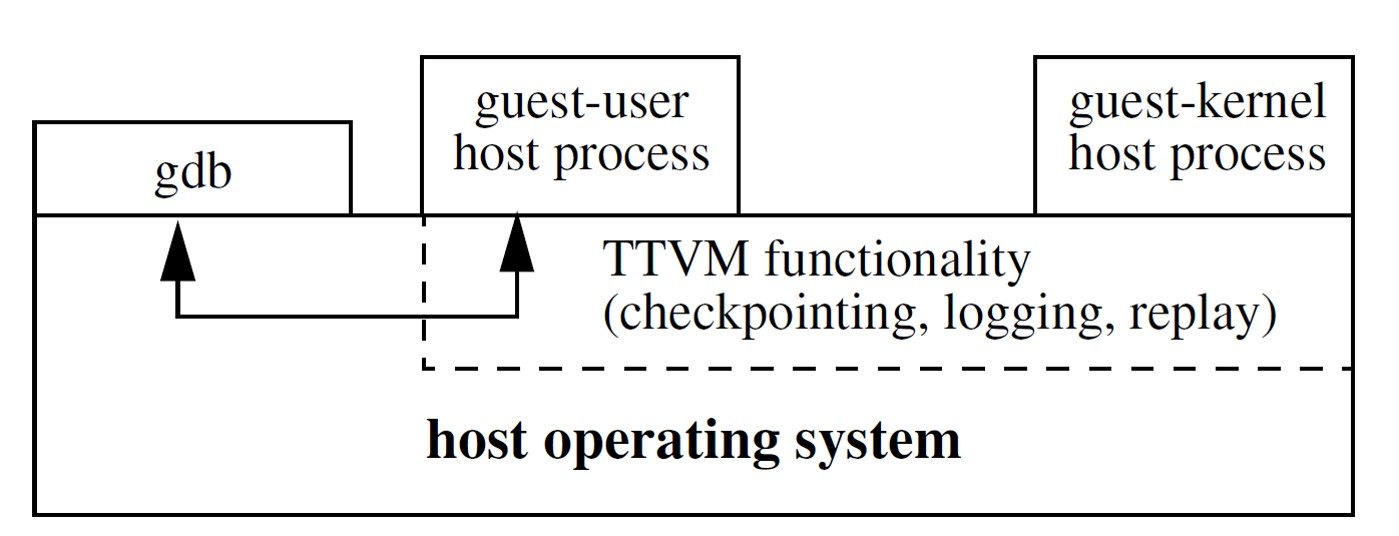
\includegraphics[height=5.5cm]{./fig2.jpg}          
\caption{System structure}
\label{fig:up}
\end{center}
\end{figure}




\section{Time-traveling vitrual machines}
\subsection{TTVM-introduction}
TTVMは2つの機能を持っている.
1つは,VMが起動してから最後の命令が実行された時までの任意の時点
の完全な状態を再現できる機能である.
2つ目は,任意の時点から実行を開始し,オリジナルの実行と同じ命令列を実行する機能である.
この章では,ロギングとリプレイ,チェックポインティングを通して,2つの機能を実装する方法を示す.

\subsection{Logging and replaying a VM}
TTVMにおける基礎的な機能は,オリジナルの実行と一致するように,与えられた時点から実行を再生する機能である.
リプレイはVMの状態とオリジナルの実行の状態を同じ状態にする.
この機能を実現するためにTTVMではReVirtというロギング/リプレイの機能を使っている.
VMMは非決定的な割り込みなどの操作を再現する.
オリジナルの実行からデバイスを読む呼び出しをロギングすることと,リプレイ実行から同じデータを
再現することで割り込み操作を再現できる.
ロギングした点は,実行が始まってからの分岐回数と,割り込み命令のアドレスによって一意に決められる.


\subsection{Host device drivers in the guest OS}
一般的には,VMMは限られた仮想デバイスのセットを提供している.
いくつかのVMMはハードウェアに存在するデバイスを提供しており,
それ以外のVMMはハードウェアに存在しないものも提供している.
限られたデバイスのセットを提供することはたいていVMの利点とみなせる.
なぜなら無数のホストOSのデバイスドライバへ対応しなくてもよいためである.
しかし,OSのデバッグの際にはこの限定されたセットはデバイスのデバッグや
デバイスを使う際の障害となる.
提供されたデバイスドライバしか使用できないためである.
この問題を解決するためにソフトウェアエミュレータが対象のデバイスに存在しない場合でもゲストOSで実ドライバを
走行させる方法を実現する.

\subsection{Checkpointing for faster time travel}
VMM起動時点からのロギングとリプレイは,実行中のほかの時点から実行中の任意の時点での
状態を再作成するのに十分である.
しかし,ロギングまたはリプレイの単独での実行はすぐにこの状態を再生するのに十分ではない.
仮想マシンが必要なポイントに最初から各命令を実行する必要があり,
この期間は何日にまたがる可能性があるためである.
長期間にわたるタイムトラベルを素早く実行するため,TTVMは定期的にチェックポイントを取る.
一番簡単な方法はVMの状態を完全にコピーすることである.
完全なコピーを取ることは簡単であるが,効率的ではない.
オーバヘッドを削減するためにcopy-on-writeとversioningという機能を使う.
前のチェックポイントから変更されたメモリページのみを保存している.
前のチェックポイントの状態の復元はアンドゥログを用いて行う.
チェックポイントnのアンドゥログにはチェックポイントnとチェックポイントn+1での変更点の
メモリセットが含まれている.
また,TTVMには次のチェックポイントへ進むためのリドゥログも実装されている.
チェックポイントnのリドゥログにはチェックポイントn-1とチェックポイントnの変更点の
情報を含んでいる.
もし連続する2つのチェックポイントのインターバルでメモリマップが書き換えられたら,
2つのインターバルの間のチェックポイントのアンドゥログとリドゥログは同じ値を持つことがある.
TTVMではこの状態を見つけだし,アンドゥログとリドゥログでその値を共有させる.
図2ではリドゥログのAとアンドゥログのAが同じ値を持っているため,この値を共有している.

\begin{figure}[t]
\begin{center}
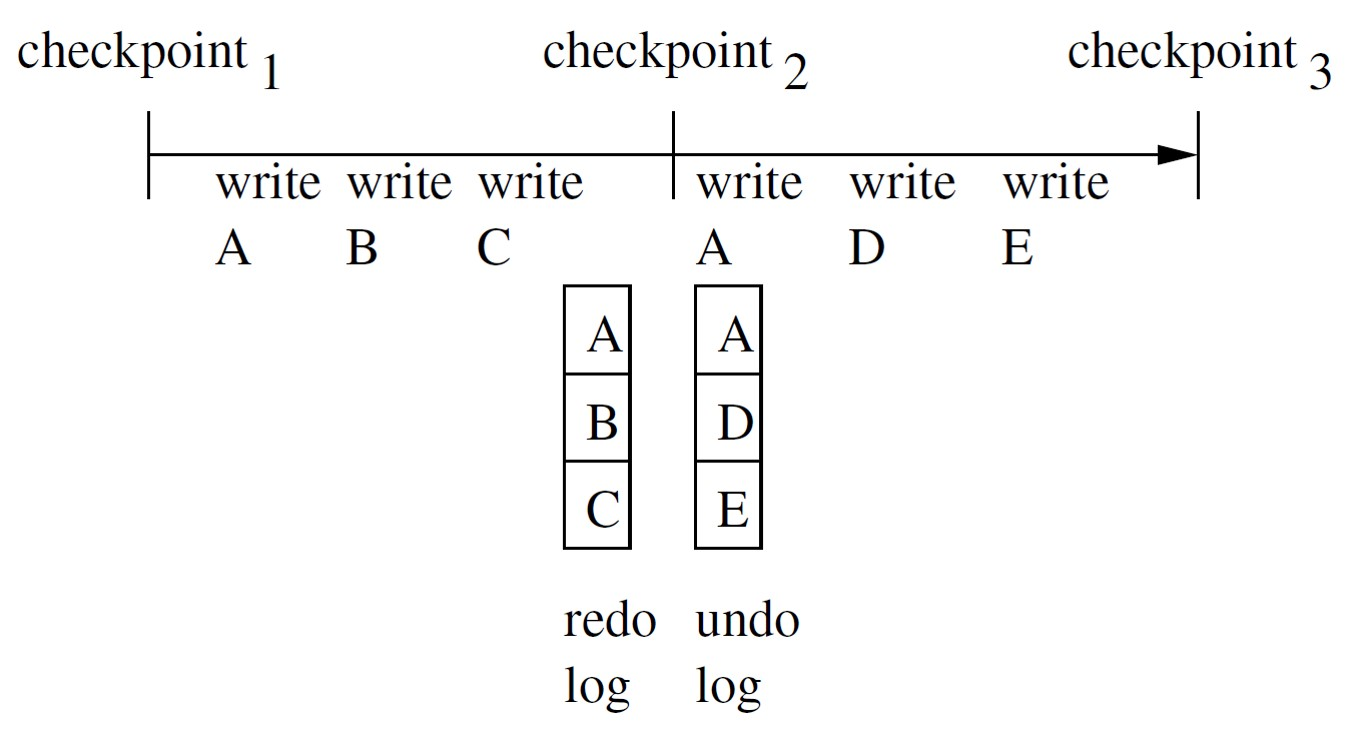
\includegraphics[height=5.5cm]{./fig1.jpg}          
\caption{Checkpoint}
\label{fig:up}
\end{center}
\end{figure}


\section{おわりに}
設計の途中までを読解した.
従来のOSデバッグの問題点と,TTVMのタイムトラベル機能の概要を理解した.
引き続き読解を進め,機能の詳しい部分の理解を深める.




\begin{thebibliography}{9}
\bibitem{bib1} Samuel, T.K., George, W.D. and Peter M.C.: Debugging operating systems with time-
travelling virtual machines, Proceedings of The USENIX Annual Technical Conference,
pp.1-15(2005).
\end{thebibliography}

\end{document}
